\documentclass{article}

\usepackage{graphicx}
\usepackage{tikz}
\usepackage{tikzsymbols}
\usetikzlibrary{calc,patterns,shapes.geometric}
\pagestyle{empty}
\usepackage[margin=0pt]{geometry}
\geometry{papersize={14in,12in}}

\def\centerarc[#1](#2)(#3:#4:#5){\draw[#1] ($(#2)+({#5*cos(#3)},{#5*sin(#3)})$) arc (#3:#4:#5);}

\begin{document}
	\begin{figure}
		\centering
		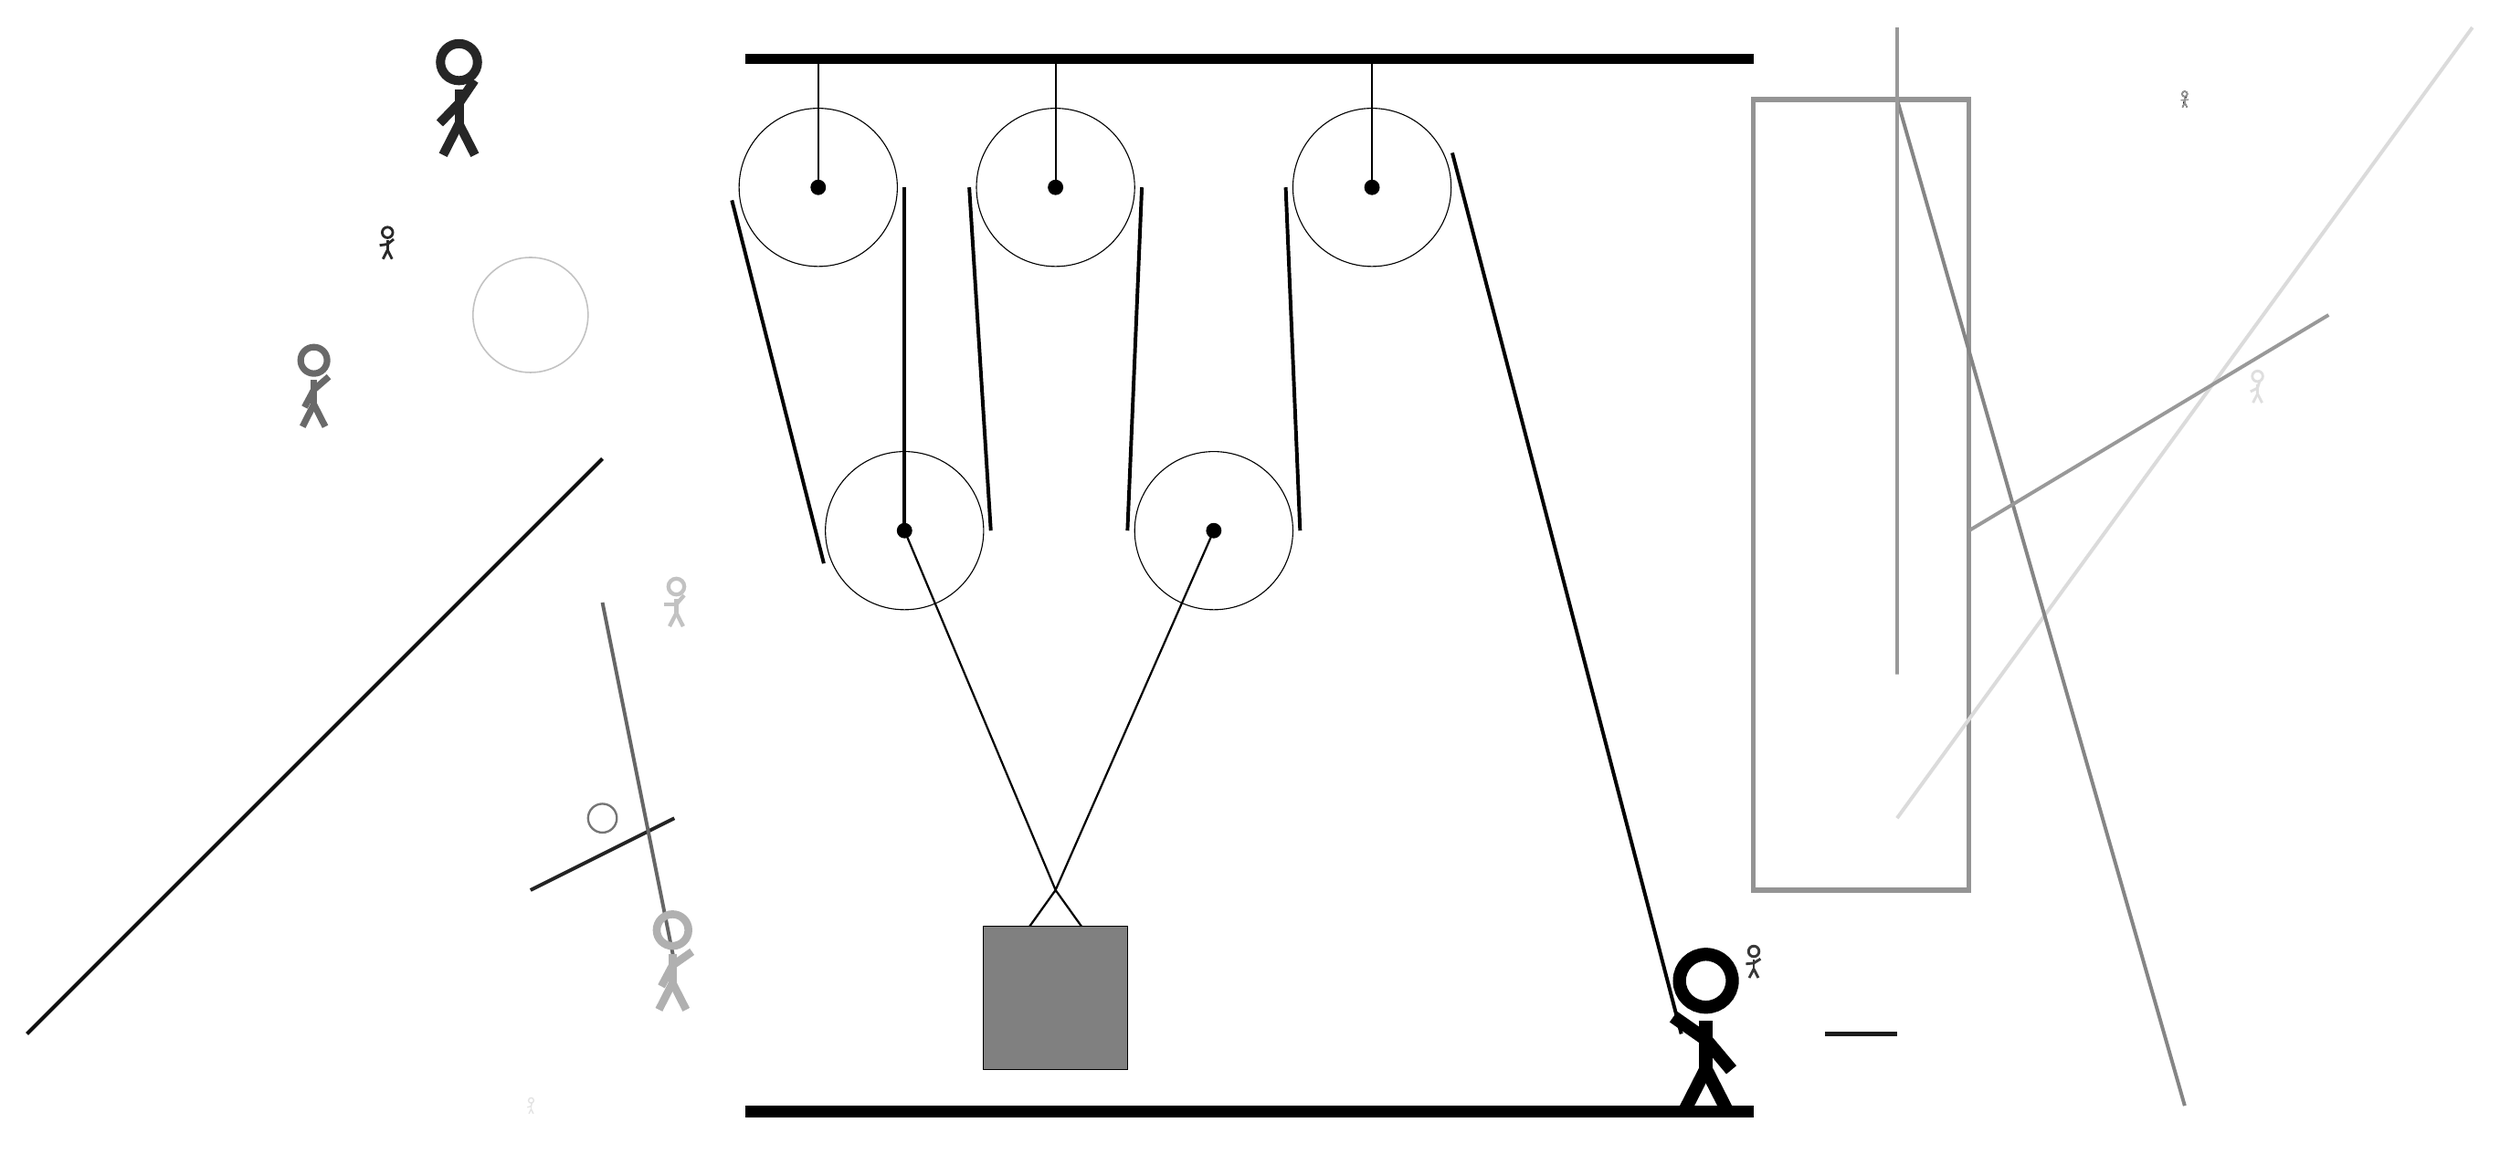
\begin{tikzpicture}
			%%%%% START %%%%%
			
			\draw[fill=black] (-2, 11.5) rectangle (12, 11.625);
			
			\draw (-1, 9.775) circle (1.1);
			\draw[fill=black] (-1, 9.775) circle (0.1);
			\draw[thick] (-1, 9.775) -- (-1, 11.5);
			
			\draw (2.3, 9.775) circle (1.1);
			\draw[fill=black] (2.3, 9.775) circle (0.1);
			\draw[thick] (2.3, 9.775) -- (2.3, 11.5);
			
			\node[line width=0.5mm, color=black!85] at (-6, 11) {\Strichmaxerl[7][46][56]};
			
			\node[line width=0.6mm, color=black!11] at (-5, -3) {\Strichmaxerl[1][14][78]};
			\draw[line width=0.7mm, color=black!42] (12, 0) rectangle (15, 11);
			\node[line width=0.3mm, color=black!13] at (19, 7) {\Strichmaxerl[2][27][73]};
			\draw[line width=0.5mm, color=black!86](-5, 0) -- (-3, 1);
			\node[line width=0.2mm, color=black!89] at (18, 11) {\Strichmaxerl[1][72][67]};
			\node[line width=0.3mm, color=black!78] at (12, -1) {\Strichmaxerl[2][6][32]};
			
			\draw[line width=0.5mm, color=black!14](14, 1) -- (22, 12);
			\node[line width=0.6mm, color=black!42] at (18, 11) {\Strichmaxerl[1][6][3]};
			\node[line width=0.3mm, color=black!24] at (-3, 4) {\Strichmaxerl[3][0][49]};
			
			\draw[line width=0.5mm, color=black!48](14, 11) -- (18, -3);
			\node[line width=0.5mm, color=black!59] at (-8, 7) {\Strichmaxerl[5][62][41]};
			\node[line width=0.3mm, color=black!84] at (-7, 9) {\Strichmaxerl[2][8][39]};
			
			\draw [line width=0.2mm, color=black!24](-5, 8) circle (0.8);
			\draw [line width=0.3mm, color=black!54](-4, 1) circle (0.2);
			\draw[line width=0.6mm, color=black!89] (13, -2) rectangle (14, -2);
			
			\draw[line width=0.5mm, color=black!60](-3, -1) -- (-4, 4);
			\draw[line width=0.5mm, color=black!94](-4, 6) -- (-12, -2);
			\draw[line width=0.5mm, color=black!40](15, 5) -- (20, 8);
			
			\node[line width=0.2mm, color=black!31] at (-3, -1) {\Strichmaxerl[6][62][35]};
			\draw[line width=0.6mm, color=black!40] (14, 3) rectangle (14, 12);
			
			
			\draw (6.7, 9.775) circle (1.1);
			\draw[fill=black] (6.7, 9.775) circle (0.1);
			\draw[thick] (6.7, 9.775) -- (6.7, 11.5);
			
			\draw (0.2, 5) circle (1.1);
			\draw[fill=black] (0.2, 5) circle (0.1);
			
			\draw (4.5, 5) circle (1.1);
			\draw[fill=black] (4.5, 5) circle (0.1);
			
			\draw[thick] (0.2, 5) -- (2.3, 0)  -- (4.5, 5);
			\draw[thick]  (1.8, -0.7) -- (2.3, 0) -- (2.8, -0.7);
			\draw[fill=black!50] (1.3, -0.5) rectangle (3.3, -2.5);
			
			\draw[line width=0.5mm] (0.2, 5) -- (0.2, 9.775);
			\centerarc[line width=0.5mm](-1, 9.775)(0:200:1.2000000000000002);
			\draw[line width=0.5mm] (-2.2, 9.595) -- (-0.922, 4.544);
			\centerarc[line width=0.5mm](0.2, 5)(200:360:1.2000000000000002);
			\draw[line width=0.5mm](1.4, 5) -- (1.1, 9.775);
			\centerarc[line width=0.5mm](2.3, 9.775)(0:180:1.2000000000000002);
			\draw[line width=0.5mm] (3.5, 9.775) -- (3.3, 5);
			\centerarc[line width=0.5mm](4.5, 5)(180:360:1.2000000000000002);
			\draw[line width=0.5mm] (5.7, 5) -- (5.5, 9.775);
			\centerarc[line width=0.5mm](6.7, 9.775)(20:180:1.2000000000000002);
			\draw[line width=0.5mm](7.816, 10.255)  -- (11, -2);
			
			\node at (11.3, -2) {\Strichmaxerl[10][-35][-50]};
			
			\draw[fill=black] (-2, -3) rectangle (12, -3.15);
			
			%%%%% END %%%%%
		\end{tikzpicture}
	\end{figure}	
\end{document}